To numerically solve a set of PDEs, iterative methods (finite difference, finite volume or finite element methods) are frequently used to approximate the solution through a discretized (step by step) phenomena. Thus, the continuous time and space domains are discretized so that a set of numerical computations are iteratively (time discretization) applied onto a mesh (space discretization). In other words, the PDEs are transformed to a set of numerical computations applied at each time step on all elements of the discretized space domain. Among those numerical computations is found a set of numerical schemes, also called \textit{stencil computations}, and a set of auxiliary computations also needed to perform the simulation, and also called \emph{local computations}.
This section gives formal definitions of a \textit{stencil program} and its computations. Then, the different parallelization techniques which can be applied on such program, are presented.

%-------------------------------------
\subsection{Time, mesh and data}

A mesh $\mathcal{M}$ defines the discretization of the continuous space domain $\Omega$ of a set of PDEs and is defined as follows. 

\begin{mydef}
\textit{A mesh is a connected undirected graph $\mathcal{M}=(V,E)$, where $V\in \Omega$ is the set of vertices and $E\in V^2$ the set of edges. The set of edges $E$ of a mesh $\mathcal{M}=(V,E)$ does not contain bridges.}
\end{mydef}
\begin{figure}[!h]\begin{center}
  \resizebox{8cm}{!}{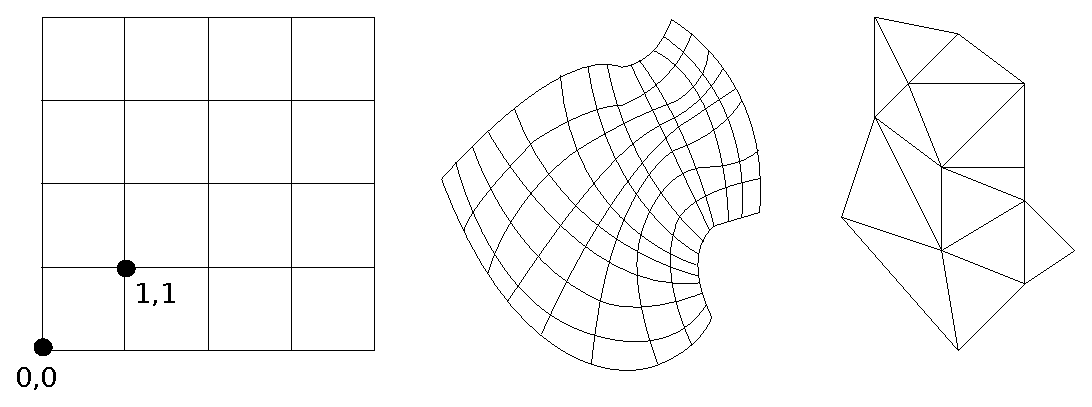
\includegraphics{./images/maillages.pdf}}
  \caption{From left to right, Cartesian, curvilinear and unstructured meshes.}
  \label{fig:mesh}
\end{center}\end{figure}
A mesh can be structured (as Cartesian or curvilinear meshes), unstructured, regular or irregular (without the same topology for each element) and hybrid. 

%\rmq{Pas très clair la suite; motivation? dom == some sub elements of M ?}
For simulations, data is discretized based on the mesh; but for a given mesh, there are various ways of mapping the data depending on the mesh entities on which the data is mapped.
\begin{mydef}
\todo{JB: vraiment, ta def dit que pour chaque couple (noeud, arete), tu associes un element de $D_i$ ...}
$D_i$ is a set of elements of a mesh $\mathcal{M}=(V,E)$, constructed by a function $dom_i$ which defines a precise association between $V$ and $E$, $dom_i : V \times E \rightarrow D_i$.
\end{mydef}

\begin{mydef}
\todo{JB: def alternative}
An entity $d$ of a mesh $\mathcal{M}=(V,E)$ is a subset of the mesh elements: $d\subset (V\cup E)$.
A kind of mesh entities $D$ is a set of entities: $D\subset \mathcal{P}(V\cup E)$
\end{mydef}
For example, in a 2D Cartesian mesh a first kind of entities are the cells ($D_0$), they can be defined as all sets containing exactly four vertices and four edges connected as a cycle. Another kind of entities are the vertices ($D_1$) that can be defined as all singletons formed of a single vertex each.

This covers the space discretization, however another dimension manipulated in simulations that has to be discretized is the time dimension.
\begin{mydef}
The discretization of the continuous time domain $\mathcal{T}$ is denoted $T$ such that $\forall\mbox{ }t_i\mbox{, }t_{i+1} \in T\mbox{, }\exists\mbox{ }\Delta t \in \mathbb{R}$\mbox{, }$t_{i+1} = t_i + \Delta t$.
\end{mydef}
$T$ is responsible for the iteration time steps of the numerical simulation. 

In a numerical simulation a set of data elements, or quantities, are applied onto the mesh and represent the set of values to compute, or to use, for computation.
\begin{mydef}
A quantity is a function $\delta_t: D_{\delta t} \mapsto V_{\delta t}$ which associates each entity of its definition domain $d\in D_{\delta t}$ to a value $v\in V_{\delta t}$ where $V_{\delta t}$ is the data type, typically $\mathbb{R}$ or $\mathbb{C}$.
The set of quantities applied on the mesh is denoted $\Delta$.
In the rest of this paper, the entities on which a quantity $\delta_t$ is mapped is denoted $dom(\delta_t)=D_{\delta t}$.
\end{mydef}
Another approach closer to that taken in applied mathematics would have been to define $\delta$ functions over $D \times T$; however the approach chosen in this paper where a distinct function is defined for each time-step better matches the implementation of numerical simulations where the outer loop iterates over time and where only a few time-steps of quantity values are stored.

%-----------------------
\subsection{Computations}

\begin{mydef}
A numerical expression $\text{exp}_{wt}: dom(w_t)\times R\mapsto V_{wt}$ is a function that computes the value of a quantity $w_t(d)$ (write quantity) for a given entity $d \in dom(w_t)=D$, using the set of its input data $R=\{\delta 1_{t-1}, \delta 2_{t-1}, ...\} \subset \Delta$ (read quantities). It is defined as $\text{exp}_{wt}(d,r) \rightarrow w_t(d)$.
\todo{JB: tu n'introduis pas la notion de stencil ici?}
\end{mydef}

\begin{mydef}
A computation $c$ of a numerical simulation is defined as $c(R,w,\text{exp})$, where $R \subset \Delta, w \in \Delta$ and $\text{exp}$ a numerical expression. %$D$ is one of the subsets $D_i \subset \mathcal{M}$, such that $w : D \rightarrow V$.
\end{mydef}
It has to be noticed that at each time iteration, all the values of a quantity are computed. However, it happens that computations of the quantity is split in different domains, as for example the computation of the physical border. In this case additional $D_i$ can be specified for the mesh $\mathcal{M}$.
\todo{JB: je comprends pas vraiment...}

\begin{mydef}
The set of $n$ ordered computations of a numerical simulation is denoted $\Gamma = [c_i]_{0 \leq i \leq n-1}$, such that $\forall c_i,c_j \in \Gamma$, if $i \leq j$, then $c_i$ is computed before $c_j$, and $c_j$ can be computed only when $c_i$ is finished.
\todo{JB: je dirais que $c_j$ peut etre calculé quand $c_j$ l'est, j'eleverais le "only", c'est justement parce qu'il n'y a pas le only que tu peux faire du task parallelism}
\end{mydef}

%JB: fin de relecture

\begin{mydef}
A \textit{multi-stencil program} is defined by the quadruplet $\mathcal{MSP}(T,\mathcal{M},\Delta,\Gamma)$.
\end{mydef}
%If the number of computations in $\Gamma$ is $card(\Gamma)=n$, such that $\bigcup_{i=0}^{n-1}c_i = \Gamma$, then $\bigcup_{i=0}^{m-1}R_i \cup w_i \subseteq \Delta$.

As already mentioned, the ordered list $\Gamma$ can be composed of two different types of computations, stencil and local computations, which will be defined in the rest of this Section.

\begin{mydef}
The neighborhood $\mathcal{N}$ of an element $d \in D_i$ is a function to obtain a set of elements in any $D_k \subset \mathcal{M}$, $\mathcal{N} : D_i \rightarrow D_k \times D_k \times \dots$.
\end{mydef}
The function $\mathcal{N}$ is also sometimes called the \textit{stencil shape}, or the \textit{stencil} in applied mathematics. In this paper we distinguish a stencil shape from a \textit{stencil computation} defined as followed:

\begin{mydef}
A \textit{stencil computation} is defined as a quadruplet $s(R,w,\text{exp},\mathcal{N})$, where $R \subset \Delta$, and $w : D \rightarrow V \in \Delta$.
\end{mydef}
In a stencil computation $s$, $\forall d \in D$, the stencil numerical expression $\text{exp}$ is applied such that $w(d) = \text{exp}(R(d),R(\mathcal{N}(d))$. In this work, a stencil computation $s(R,w,\text{exp},\mathcal{N})$ always verifies $R \cap \{w\} = \emptyset$, otherwize an implicit numerical scheme has to be solve which is over the scope of this paper. As a result, the ordered list $\Gamma$ of a multi-stencil program can be composed of a set of stencil computations applied on one or more stencil shapes.

Figure~\ref{fig:ex} gives an example of a stencil computation $s(R,w,\text{exp},\mathcal{N})$, where $\mathcal{M}(V,E)$ is a two dimensional Cartesian mesh. A single domain $D=dom(w)$ is defined in this example and is composed of cells formed by a cycle of four vertices $v \in V$ and four edges $e \in E$. Furthermore, in this example $R=\{A\}$, $w=B$, and for $(x,y) \in D$ the neighborhood function is 
\begin{equation*}
\mathcal{N} : (x,y) \rightarrow \{(x,y+1),(x,y-1),(x+1,y),(x-1,y)\}.
\end{equation*}
Finally, the numerical expression of this example is 
\begin{equation*}
\text{exp}(A(x,y),A(\mathcal{N}(x,y)) = B(x,y) = A(x,y)+(A(x,y+1)+A(x,y-1)+A(x+1,y)+A(x-1,y))/4.
\end{equation*}

\begin{figure}[!h]\begin{center}
  \resizebox{8cm}{!}{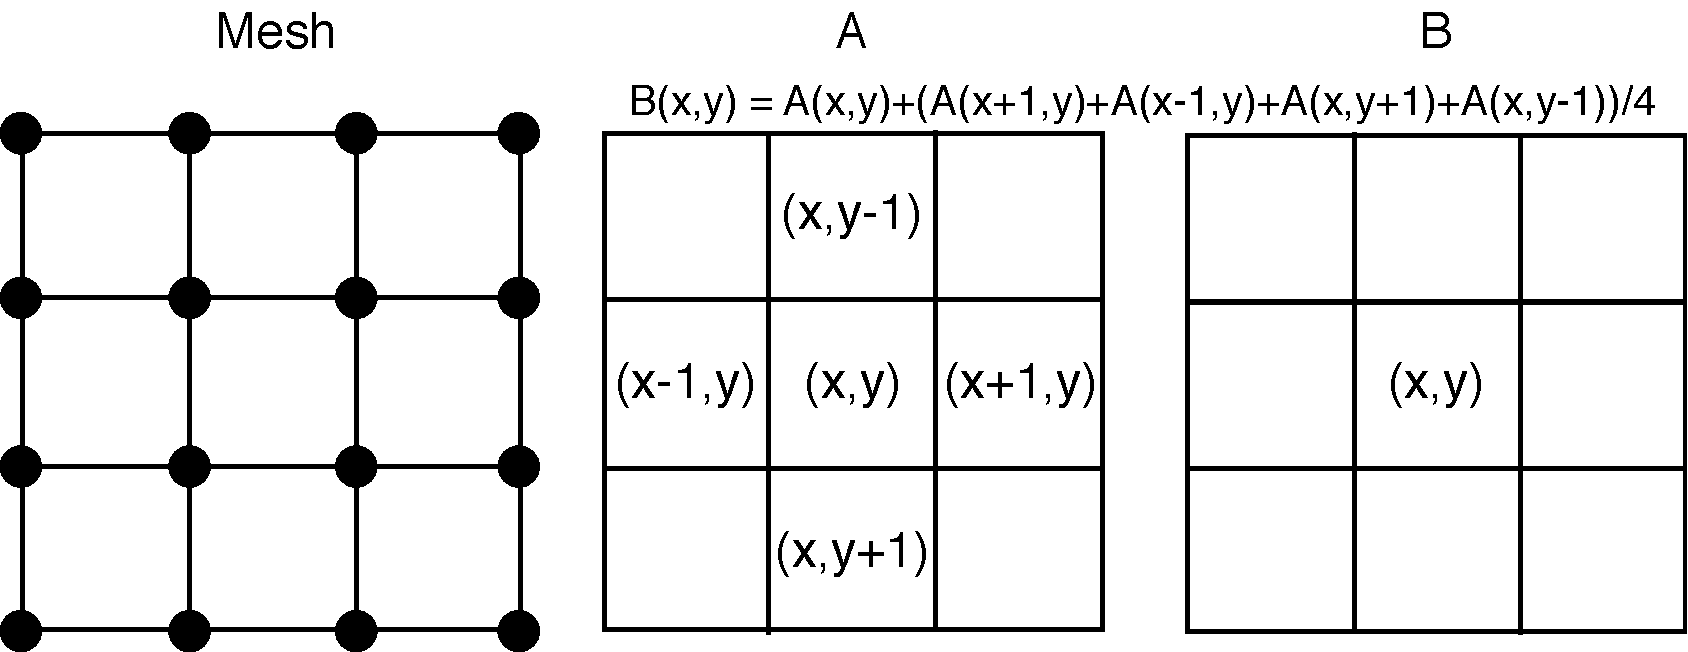
\includegraphics{./images/example.pdf}}
  \caption{Example of a stencil computation.}
  \label{fig:ex}
\end{center}\end{figure}

The second type of numerical computation is a local computation.
\begin{mydef}
A local computation is a triplet $l(R,w,\text{exp})$, where $exp$ does not involve a neighborhood function $\mathcal{N}$.
\end{mydef}

A stencil program and stencil and local computations have been formally defined in this section. This formalism is used in the next Section to define two parallelization techniques of a multi-stencil program.


